\chapter{Biological effects of radiation \label{chap:biol}}

Radiation which interacts with electrons can affect chemical bonds in
DNA, and as a result, cause damage to living tissues. The probability
that an elementary particle will cause an adverse ionisation is
proportional to the energy of the particle deposited in the tissue. In
addition, the damage done per unit energy depends on the type of
particle.

In diagnostic nuclear medicine, the aim is of course to obtain
diagnostic images without or with minimum damage to the
patient. Consequently, the amount of activity administered to the
patient should be as low as reasonably achievable (ALARA).
``Reasonably achievable'' means that the radiation emitted by the
tracer should still be sufficient to make valuable clinical images.

The amount of radiation deposited in an object is expressed in gray (Gy). A
dose of 1 gray is defined as the deposition of 1 joule per kg absorber:
\begin{equation}
  1 Gy = 1 \frac{J}{kg}.
\end{equation}

To quantify (at least approximately) the amount of damage done to living
tissue, the influence of the particle type must be included as well. E.g. it
turns out that 1 J deposited by neutrons does more damage than the same energy
deposited by photons. To take this effect into account, a quality factor $Q$
is introduced. Multiplication with the quality factor converts the dose into
the dose equivalent. Quality factors are given in table \ref{tab:qualfactor}.
%
\begin{table}[h]
\begin{center}
\caption{Quality factor converting dose in dose equivalent (ICRP2007).
\label{tab:qualfactor}}
\begin{tabular}{|l|c|}
\hline
Radiation                          & Q \\
\hline
\hline
X-ray, $\gamma$-ray,               & \\
electrons, positrons               & 1 \\
\hline
protons                            & 2 \\
neutrons                           & 2.5 \ldots 22, depending on energy \\
\hline
$\alpha$-particals                 & 20 \\
\hline
\end{tabular}
\end{center}
\end{table}


The dose equivalent is expressed in Sv (sievert). Since $Q = 1$ for photons,
electrons and positrons, we have 1 mSv per mGy in diagnostic nuclear
medicine. The natural background radiation is about 2 mSv per year, or
about 0.2 $\mu$Sv per hour.\\

The older units for radiation dose and dose equivalent are rad and rem:
\begin{eqnarray}
  \mbox{1 Gy} & = & \mbox{100 rad}\\
  \mbox{1 Sv} & = & \mbox{100 rem}
\end{eqnarray}

When the dose to every organ is computed, one can in addition compute
an ``effective dose'', which is a weighted sum of organ doses. The
weights are introduced because damage in one organ is more dangerous
than damage in another organ. The most sensitive organs are the gonads
(weight about 0.25), the breast, the bone marrow and the lungs (weight
about 0.15), the thyroid and the bones (weight about 0.05), see table
\ref{tab:effdose}. The sum of all the weights is 1. The weighted
average produces a single value in mSv. The risk of death due to tumor
induction is about 5\% per ``effective Sv'' according to report
ICRP-60 (International Commission on Radiological Protection
(http://www.icrp.org)), but it is of course very dependent upon age
(e.g. 14\% for children under 10). Research in this field is not
finished and the tables and weighting coefficients are adapted every
now and then.

\begin{table}[h]
\begin{center}
\caption{Organ weight factors to compute the effective dose (ICRP 103, 2007).
\label{tab:effdose}}
\begin{tabular}{|c|c|c|}
  \hline
  organ & weight & total\\
  \hline
  red marrow, colon, lungs, stomach, breast & 0.12 & 0.60\\
  \hline
  gonads & 0.08 & 0.08\\
  \hline
  bladder, liver, esophagus, thyroid & 0.04 & 0.16\\
  \hline
  brain, skin, salivary glands, bone surfaces & 0.01 & 0.04\\
  \hline
  remainder (adrenals, extrathoracic region, & & \\
  gallbladder, heart, kidneys, lymphatic nodes, & 0.00923& 0.12\\
  muscle, oral mucosa, pancreas, prostate, & & \\
  small intestine, spleen, thymus, uterus/cervix) & &\\
  \hline
  total  & & 1 \\
  \hline
\end{tabular}
\end{center}
\end{table}


To obtain the dose equivalent delivered by one organ $A$ to another organ $B$
(or to itself, in which case $A = B$), we have to make the following
computation:
\begin{equation}
  \mbox{DE} = \sum_i Q_i \;\times\; N_{iA} \;\times\; p_i(A \rightarrow B) 
               \;\times\; E_i \;/\; M_B, \label{eq:DE}
\end{equation}
\begin{description}
  \item[DE] is the dose equivalent;

  \item[$i$] denotes a particular emission. Often, multiple photons or
            particles are emitted during a single radioactive event, and we
            have to compute the total dose equivalent by summing all
            contributions;

  \item[$Q_i$] is the quality factor for emission $i$;

  \item[$N_{iA}$] is the total number of particles $i$ emitted in organ $A$;

  \item[$p_i(A \rightarrow B)$] is the probability that a particle $i$ emitted
       in organ $A$ will deposit (part of) its energy in organ $B$;

  \item[$E_i$] is the (average) energy that is carried by the particles $i$ and
       that can be released in the tissue. For electrons and positrons, this is
       their kinetic energy. For photons, it is all of their energy.

  \item[$M_B$] is the mass of organ $B$.
\end{description}
In the following paragraphs, we will discuss these factors in more detail, and
illustrate the procedure with two examples.

\section{The particle $i$}
%=========================
The ideal tracer for single photon emission would emit exactly one photon in
every radioactive event. However, most realistic tracers have a more complex
behaviour. Some of them emit several photons at different energies and in
different quantities. For example, Iodine-123 has several different ways of
decaying (via electron capture) from $^{123}_{53}$I into $^{123}_{52}$Te.
Each decay scheme produces its
own set of photons. Most of these schemes share an energy jump of 159 keV, and
the mean number of 159 keV photons emitted per desintegration equals
0.836. In some of the decay schemes, there is an internal conversion electron
with an average energy of 127 keV, that comes with a probability of 0.134 per
desintegration. In total,
$^{123}_{53}$I uses combinations of 14 different gamma rays, 5 x-rays, 3
internal conversion electrons and 5 Auger electrons to get rid of its excess
energy. Each of those has its own probability. In principle, we need to
include them all, but it usually suffices to include only the few dominating
emissions.

\section{The total number of particles $N_{iA}$}
%=========================
The number of particles emitted per s changes with time. Due to the finite
half life, the radioactivity decays exponentially (see eq
(\pref{jn:decay})). Moreover, the distribution of the tracer molecule in the
body is determined by the metabolism, and it changes continuously from the
time of injection. Often, the tracer molecule is metabolized: the molecule is
cut in pieces or transformed into another one. In those cases, the radioactive
atoms may follow one or several metabolic pathways. As a result, it is often
very difficult or simply impossible to accurately predict the amount of
radioactivity in every organ as a function of time. When a new tracer is
introduced, the typical time-activity curves are mostly determined by repeated
emission scans in a group of subjects.

Assuming that we know the amount of radioactivity as a function of time, we
can compute the total number of particles as
\begin{equation}
  N_{iA} =  \int_0^{\infty} n_{iA}(t) dt,
\end{equation}
where $n_{iA}(t)$ is the number of particles emitted per s at time $t$.
For some applications, it is reasonable to assume that the tracer behaviour is
dominated by its physical decay. Then we have that
\begin{eqnarray}
  N_{iA} & = & n_{iA}(0) \int_0^{\infty} e^{- \ln(2) \frac{t}{t_{1/2}}} dt \nonumber\\
         & = & n_{iA}(0) \frac{t_{1/2}}{\ln(2)}. \label{eq:biol_decay}
\end{eqnarray}
Here $n_{iA}(0)$ is the number of particles or photons emitted per s at time
0, and $t_{1/2}$ is the half life.
For a source of 1 MBq at time 0, $n_{iA}(0) = 10^6$ per s, since 1 Bq is
defined as 1 emission per s.

Often, the tracer is metabolized and sent to the bladder, which implies a
decrease of the tracer concentration in most other organs. Therefore,
the amount of radioactivity decreases faster than predicted by
(\ref{eq:biol_decay}) in these organs. One way to approximate the combined
effect of metabolism and physical decay could be to replace the physical
half life with a shorter, effective half life in (\ref{eq:biol_decay}).
In other cases, it may
be necessary to integrate the measured time activity curves numerically.

\section{The probability $p_i(A \rightarrow B)$}
%=========================
This probability depends on the geometric configuration of the organs
and on the attenuation coefficients. The situation is very different
for photons on the one hand and electrons and positrons on the
other. As illustrated by table \pref{tab:positron_length} for
positrons, the mean path length of an electron and positron in tissue
is very short, even for relatively high kinetic
energies. Consequently, for these particles, $p_i(A \rightarrow A)$ is
close to 1, while $p_i(A \rightarrow B)$ is negligible for different
organs $A$ and $B$. The probability that a photon travels from A to B
depends on the attenuation along that trajectory. Similarly the
probability that it deposits all or a part of its energy in B depends
on the attenuation coefficient in organ B.


\section{The energy $E_i$}
%=========================
As mentioned above, $E_i$ denotes kinetic energy for electrons and positrons,
and the total amount of energy for photons. This energy is usually given in
electronvolt. However, to compute the result in Gy, we need the energy in joule.
The eV is defined as the amount of energy acquired by an electron if it
is accelerated in an electrical field of 1 V. Because joule equals coulomb
times volt, we have that
\begin{equation}
 1 \mbox{eV} = 1.6 \times 10^{-19} \mbox{coulomb} \times \mbox{volt}
             = 1.6 \times 10^{-19} \mbox{J}.
\end{equation}

\section{Example 1: single photon emission}
%=========================
Consider the configuration shown in fig \ref{fig:biol-singlephoton}.
Assume that the point source in the left box contains 1 MBq of the
isotope $^{123}$I. As discussed before, this isotope has a very
busy decay scheme, but we will assume that we can ignore all emissions
except the following two:
\begin{enumerate}
  \item Gamma radiation of 159 keV, with an abundance of 0.84,
  \item Conversion electron of 127 keV, with an abundance of 0.13.
\end{enumerate}
The half life of $^{123}$I is 13.0 hours.
The boxes are made of plastic or something like that, with an
attenuation coefficient of 0.15 cm$^{-1}$ for photons with energy
of 159 keV. The density of the boxes is 1 kg/liter.
The boxes are hanging motionless in air, the attenuation
of air is negligible. Our task is to estimate the dose that both boxes
will receive if we don't touch this configuration for a few days.
%
%
\begin{figure}[tb]
\centering
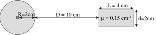
\includegraphics[width=\figmedium]{figs/fig_biol_singlephoton.pdf}
\caption{\label{fig:biol-singlephoton} \emph{Two objects, one with a
radioactive source in the center. The size of the right box is
2 $\times$ 2 $\times$ 4 cm$^3$}.}
\end{figure}

We are going to need the mass of the boxes. For the left box we
have:
\begin{equation}
  W_{\mbox{left}} = \frac{4}{3} \pi R^3 \; \times \; 1 \frac{\mbox{kg}}{\mbox{dm}^3}
      = 0.034 \;\mbox{kg},
\end{equation}
and for the right box:
\begin{equation}
  W_{\mbox{right}} = d^2 L\; \times \; 1 \frac{\mbox{kg}}{\mbox{dm}^3}
      = 0.016 \;\mbox{kg}.
\end{equation}

Because a few days lasts several half lifes, a good approximation is
to integrate until infinity using equation (\ref{eq:biol_decay}).
Consequently, the total number of desintegrations is estimated as
\begin{equation}
  N = 1 \mbox{MBq} \times \frac{13\ \mbox{hours}}{\ln(2)} 
    \times 3600 \frac{s}{\mbox{hour}}
    = 6.75 \times 10^{10}.
\end{equation}
This number must be multiplied with the mean number of particles per
desintegration:
\begin{tabbing}
  \hspace{4mm} \= number of electrons is \= 0.13 N \= = 8.78 $\times$ 10$^{9}$ \kill
               \> number of photons is \> 0.84 N \> = 5.67 $\times$ 10$^{10}$\\
               \> number of electrons is   \> 0.13 N \> = 8.78 $\times$ 10$^9$
\end{tabbing}

The radius of the left box is large compared with the mean path length
of the electrons, so the box receives all of their energy:
$p_{\beta^-}(\mbox{leftbox} \rightarrow \mbox{leftbox}) = 1$. Thus, the
dose of the left box due to the electrons is:
\begin{equation}
  \mbox{dose}(\beta^-,\mbox{leftbox}) = 8.78 \times 10^9 \; \times \; 
         127000 \ \mbox{eV} \;
    \times \frac{1.6 \times 10^{-19} \ \mbox{J}}{\mbox{eV}} \times 
          \frac{1}{0.034 \ \mbox{kg}}
      = 5 \mbox{mGy}.
\end{equation}
For the photons, the situation is slightly more complicated, because
not all of them will deposit their energy in the box. Because the box
is spherical and the point source is in the center, the amount of
attenuating material seen by a photon is the same for every direction.
With equation (\pref{jn:spectatten}) we can compute the probability that
a photon will escape without interaction:
\begin{equation}
  p_{\mbox{escape}} = e^{- \int_0^R \mu dr} = e^{- \mu R} 
     = \exp(- \frac{0.15}{\mbox{cm}} \; \times \; 2 \ \mbox{cm}) = 0.74.
\end{equation}
Thus, there is a chance of 1 - 0.74 = 0.26 that a photon will interact.
This interaction could be a Compton event, in which only a part of the
photon energy will be absorbed by the box. This complicates the computations
considerably. To avoid the problem, we will go for a simple but pessimistic
solution: we simply assume that every interaction results in a complete
absorption of the photon. That yields for the photon dose to the left box:
\begin{equation}
  \mbox{dose}(\gamma, \mbox{leftbox}) 
   =  5.67 \times 10^{10} \; \times  159\ \mbox{keV} 
    \times \frac{1.6 \times 10^{-19} \ \mbox{J}}{\mbox{eV}}
    \times \frac{1}{0.034 \ \mbox{kg}} \times \; 0.26 = 11 \mbox{mGy}.
\end{equation}
So the total dose to the left box equals about 16 mGy.

For the right box, we can ignore the electrons, they cannot get out of the
left box.  We already know that a fraction of 0.74 of the photons escapes the
left box. Now, we still have to calculate which of those will interact with
the right box. We first estimate the fraction traveling along a direction that
will bring it into the right box.  When observed from the point source
position, the right box occupies a solid angle of approximately $d^2 / (D +
R)^2$. The total solid angle equals $4 \pi$, so the fraction of photons
travelling towards the right box equals
\begin{equation}
  p_{\mbox{geometry}} = \frac{d^2}{4 \pi (D + R)^2} = 0.0022.
\end{equation}
These photons are travelling approximately horizontally, so most of them are
now facing 4 cm of attenuating material. Applying the same pessimistic
approach as above yields the fraction that interacts with the material of the
right box:
\begin{equation}
  p_{\mbox{attenuation}} = 1 - e^{- \mu L} = 0.45.
\end{equation}
Combining all factors yields then number of photons interacting with the right box:
\begin{equation}
  5.67 \times 10^{10} \times 0.74 \times 0.0022 \times 0.45 = 4.2 \times 10^7.
\end{equation}
Finally, multiplying with the energy and dividing by the mass yields:
\begin{equation}
  \mbox{dose}(\gamma, \mbox{rightbox}) = 4.2 \times 10^7\ \times 159\ \mbox{keV}
  \times \frac{1.6 \times 10^{-19} \ \mbox{J}}{\mbox{eV}}
   \times \frac{1}{ 0.016 \ \mbox{kg}}
   = 0.067 \mbox{mGy}.
\end{equation}
This is much less than the dose of the left box. The right box is protected by its
distance from the source!


\section{Example 2: positron emission tomography}
%=========================
Here, we study the same setup of fig \pref{fig:biol-singlephoton}, but
now with a point source containing 1 MBq of $^{18}$F. This is a
positron emitter. From table \pref{tab:positron_length}, we know that
the average kinetic energy of the positron is 250 keV. Most of this
energy is dissipated in the tissue before the positron
annihilates. Thus, there are three contributions to the dose of the
left box: the positron and the two photons. The right box can at most
be hit by one of the photons.
%
We assume that in every desintegration, exactly one positron is
produced, which annihilates with an electron into two 511 keV.  At 511
keV, the attenuation of the boxes is 0.095 cm$^{-1}$. The half life of
$^{18}$F is 109 minutes.

The total number of desintegrations is 
\begin{equation}
  N = 1 \mbox{MBq} \times \frac{109\ \mbox{min}}{\ln(2)} \times 60
    \frac{s}{\mbox{min}} = 9.44 \times 10^9.
\end{equation}

Proceeding in the same way as above, we find the following doses:
\begin{eqnarray}
\mbox{dose}(\beta^+,\mbox{leftbox}) & = & 9.44 \times 10^9 \; \times \; 250000
    \ \mbox{eV} \; \times \frac{1.6 \times 10^{-19} \ \mbox{J}}{\mbox{eV}}
        \times \frac{1}{0.034 \ \mbox{kg}}  \nonumber\\
     & = & 11 \mbox{mGy}.  \\
\mbox{dose}(\gamma, \mbox{leftbox}) & = & 9.44 \times 10^9 \; \times
    \; 511000 \ \mbox{eV} \;
    \times \frac{1.6 \times 10^{-19} \ \mbox{J}}{\mbox{eV}} \;
     \times \frac{1}{0.034\ \mbox{kg}} \times \; 0.17 \nonumber\\
     & = & 3.9 \mbox{mGy}.
\end{eqnarray}
The total dose then equals $\mbox{dose}(\beta^+,\mbox{leftbox}) + 2 \;
\mbox{dose}(\gamma, \mbox{leftbox})$ = 18.8 mGy.

For the right box, we first estimate the number of interacting photons
(remember that there are two photons per desintegration):
\begin{equation}
  2N \ p_{\mbox{escape}}\ p_{\mbox{geometry}}\ p_{\mbox{attenuation}}
   = 2N \times 0.83 \times 0.0022 \times 0.32 = 1.09 \times 10^7.
\end{equation}
And for the dose to the right box we get:
\begin{equation}
\mbox{dose}(\gamma, \mbox{rightbox}) = 1.09 \times 10^7\; \times \; 511000 \ \mbox{eV} \;
  \times \frac{1.6 \times 10^{-19} \ \mbox{J}}{\mbox{eV}}  \times \frac{1}{0.016\ \mbox{kg}}
   = 0.056 \mbox{mGy}.
\end{equation}


\section{Internal dosimetry calculations}
%=========================
Internal dosimetry calculations use the same principle as in the
examples above to compute the dosage to every organ. Because there are
many organs, and because the activity in any organ contributes to the
dose in any other organ, the computations are complex and tedious.
This is one of the reasons why dedicated software has been developed.
With the fast computers we have today, the calculations can be carried
out more accurately. E.g.  it is possible to take the effects of
Compton scatter into account using Monte Carlo techniques.

Of course, we still have to provide a meaningful input to the
software. In principle, we should input the precise anatomy of the
patient. Because this is usually not available, this problem is
avoided by using a few standard geometries, which model the human
anatomy, focussing on the most senstive organs. It follows that the
resulting doses should only be considered as estimates, not as
accurate numbers.

We also have to provide the tracer concentration as a function of time
for all organs.  For known tracers, the software may contain typical
residence times; for new ones, measurements in humans have to be
carried out to estimate the dosimetry.
